%!TEX root = paper.tex

\section{Methodology}\label{sec:methodology}

In this section, we present our theoretical approach for attacking the remote model and our practical methodology for developing a suitable software.
The general idea is to train a local model which approximates the behavior of the remote model such that an adversarial example created for the local model also misleads the remote one.
Thus, we first describe how we turn the remote black-box oracle into a local white-box model in Subsection~\ref{subsec:modelstealing}.
Afterwards, we attack the local model so that the generated adversarial image also transfers to the remote model, i.e., it also fools the remote model.
Therefore, we introduce the attacks for generating adversarial examples in the subsequent parts of this section.
Finally, we present our software developing methodology in Subsection~\ref{subsec:sw_development}.

\subsection{Model Stealing}\label{subsec:modelstealing}

The attacks which are introduced later in this section assume white-box access to a target model (i.e. the entire architecture including the amount of layers and neurons, the learned weights and the activation functions need to be known).
Because we are limited to a black-box access and the knowledge of the training data, we need to turn this into a white-box model.

The following discussion is based on the transferability property of adversarial examples.
It describes the observation that an adversarial example which is misclassified on one model may be misclassified by another similar model.
The transferability spans across different machine learning methods (e.g. between neural networks and support vector machines) and even works on disjoint datasets from the same underlying distribution. \cite{papernot2016transferability,goodfellow6572explaining, szegedy2013intriguing}

We can leverage the transferability property to receive white-box access to a model.
Because adversarial samples transfer between different machine learning methods, we do not need to know the exact architecture of the remote model but instead can choose our own local white-box architecture.
By training multiple neural networks with different layers, we can approximate the optimal architecture.
To extract the information from the remote model, we can further take advantage of the transferability property in two different ways:

\begin{enumerate}
\item[1.] \textbf{Rebuilding}

We train a local model on the GTSRB dataset which we will refer to as gtsrb model throughout this paper.
This training exploits the fact that adversarial examples transfer between models which have been trained on the same underlying distribution.

\item[2.] \textbf{Training a Substitute}

By feeding the GTSRB dataset to the remote model, we can collect the classification results, which can be used to train a substitute model \cite{tramer2016stealing}.

A more sophisticated method is the Jacobian-based dataset augmentation where the decision boundary is extracted by selectively querying the oracle along the gradient \cite{papernot2017practical}.
\end{enumerate}

\begin{figure}
	%!TEX root = paper.tex
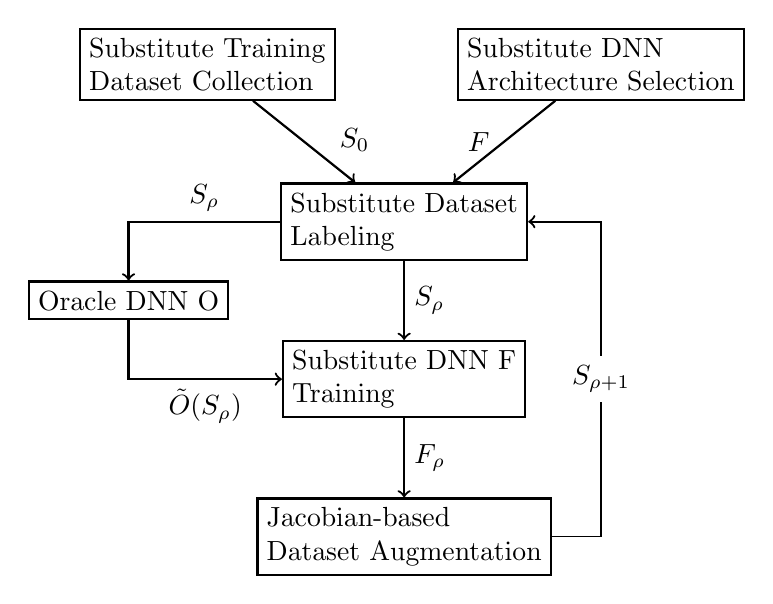
\begin{tikzpicture}[node distance = 2cm, auto]
    \node [rectangle, thick, draw, align=left] (init) at (1,10) {Substitute Training \\ Dataset Collection};
    \node [rectangle, thick, draw, align=left] (selection) at (6,10) {Substitute DNN \\ Architecture Selection};
    \node [rectangle, thick, draw, align=left] (labeling) at (3.5,8) {Substitute Dataset \\ Labeling};
    \node [rectangle, thick, draw, align=left] (training) at (3.5,6) {Substitute DNN F \\ Training};
    \node [rectangle, thick, draw, align=left] (augmentation) at (3.5,4) {Jacobian-based \\ Dataset Augmentation};
    \node [rectangle, thick, draw, align=left] (oracle) at (0,7) {Oracle DNN O};
    \node (helper) at (6,6) {$S_{\rho+1}$};

    \draw[->, thick] (init) -- (labeling) node [near end] {$S_0$};
    \draw[->, thick] (selection) -- (labeling) node [above,near end] {$F$};
    \draw[->, thick] (labeling) -- (training) node [midway] {$S_\rho$};
    \draw[->, thick] (training) -- (augmentation) node [midway] {$F_\rho$};
    \draw[->, thick] (labeling) -| (oracle) node [near start, above] {$S_\rho$};
    \draw[->, thick] (oracle) |- (training) node [near end, below] {$\tilde{O}(S_\rho)$};
    \draw (augmentation) -|  (helper);
    \draw[->, thick] (helper) |- (labeling);
\end{tikzpicture}
	\caption{\textbf{Basic flow of the Jacobian-based Dataset Augmentation.} \cite{papernot2017practical}}
	\label{fig:jbda}
\end{figure}

With reference to existing literature, the substitute training combined with a Jacobian-based dataset augmentation appear to be the most promising~\cite{papernot2017practical}, since \citeauthor{papernot2016cleverhans} use the same threat model with a pure black-box access.
The general idea is to replicate the remote decision boundary by following the gradient of the prediction, thus finding regions in the feature space where the remote model returns low confidences.

More precisely, the Jacobian-based dataset augmentation involves multiple training iterations, as shown in Figure~\ref{fig:jbda}.
Starting from an initial dataset $S_0$ and a selected architecture $F$, the labels of the initial iteration $\rho = 0$ are gathered.
Then, a substitute DNN $F$ is trained which is then augmented according to its Jacobian which is the gradient with respect to each input dimension.
In subsequent iterations, this dataset is further augmented until the maximum number of iterations is reached.
The substitute model which has been trained in the last iteration is the final output.

After initial experiments, we quickly noticed that the original algorithm does not produce acceptable results as-is and that it needs some refinement in our context.
Thus, we created a custom extension to this algorithm which we expect to yield a better approximation of the remote decision boundary.
As previously described, the original Jacobian-based dataset augmentation takes a single image per class, fetches the remote labels, trains an intermediate model on this data and computes new synthetic data points along the gradient of the local model.
We found it problematic that first, this does not handle low-confidence source samples very well: The intermediate model can be hardly trained on these inputs.
Second, the original algorithm starts at an unknown confidence and generates new data in both the positive and negative gradient direction.
It is parameterized by a number of iterations $\rho$ and a step size $\lambda$ which are fixed for all classes.
Obviously the combination of an unknown starting point and a fixed step size in both directions is counter productive, since this can easily lead to generated images which are off the manifold and there is no way to control how many of these samples are generated.

To cope with these flaws, we modified the algorithm such that it starts with a specified number of input samples per class, which are guaranteed to be classified with a higher confidence than a certain threshold.
After that, our modified version only generates synthetic data along the negative gradient.
This reflects starting at the peak for each class and systematically exploring the path towards the minimum confidence of the model.
We also noticed that some classes never result in high confidence predictions which is why we introduced a third variable limiting the number of tries to fetch high confidence samples.
The modified algorithm always keeps track of the best samples fetched so far which are taken if the maximum number of tries has been reached.
This limit is important due to the enforced request delay of one second between each prediction on average.
The number of samples per class, the confidence threshold as well as the maximum number of tries per class and sample are configurable parameters in our algorithm.
Notably, by parameterizing the number of starting images per class, we improved the initial intermediate model's training results. 
Facing 43 classes (or 36 in the reduced dataset as discussed below), the training on single images per class hardly ever converged.
Moreover, we wanted to prevent overfitting on certain source images and their synthetic derivatives by this measure, since there are also different angles and lighting settings in the reference dataset.

\begin{figure}
\begin{subfigure}{.19\linewidth}

\includegraphics[width=0.7\linewidth]{imgs/missing/00000_00012}
\end{subfigure}
\begin{subfigure}{.19\linewidth}
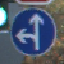
\includegraphics[width=0.7\linewidth]{imgs/missing/00001_00016}
\end{subfigure}
\begin{subfigure}{.19\linewidth}
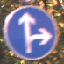
\includegraphics[width=0.7\linewidth]{imgs/missing/00001_00027}
\end{subfigure}
\begin{subfigure}{.19\linewidth}
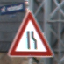
\includegraphics[width=0.7\linewidth]{imgs/missing/00001_00026}
\end{subfigure}
\begin{subfigure}{.19\linewidth}
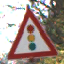
\includegraphics[width=0.7\linewidth]{imgs/missing/00003_00021}
\end{subfigure}%
\begin{subfigure}{.19\linewidth}
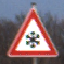
\includegraphics[width=0.7\linewidth]{imgs/missing/00004_00016}
\end{subfigure}
\begin{subfigure}{.19\linewidth}
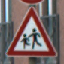
\includegraphics[width=0.7\linewidth]{imgs/missing/00014_00027}
\end{subfigure}
\caption{Training images missing from the remote model's classifications}
\label{fig:missing}
\end{figure}

Given the fact that the remote model has been trained on the GTSRB dataset, we hypothesized that it should be able to predict all occurring classes.
We therefore chose to crawl each image of the dataset once and cache the predictions in a python pickle file.
Lastly, we analyzed the results and recognized that there are seven classes of GTSRB that never occur in the classification output of the remote model as shown in Figure \ref{fig:missing}.
Also, the cached dataset predictions are the basis for a static map which translates the class numbers and names of the local dataset to the ones returned by the remote model.
Concluding that it would be not sensible to target the missing classes, we excluded them from all further considerations.


\begin{figure}
	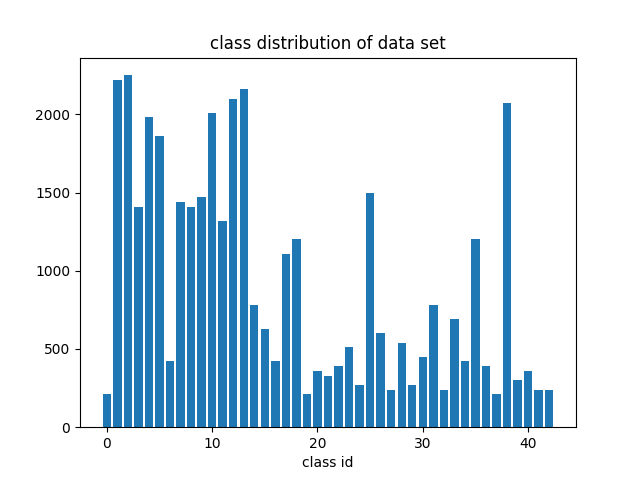
\includegraphics[width=1.1\linewidth]{figs/class_distr}
	\caption{The class ditribution of the GTSRB dataset.}
	\label{fig:class_distr}
\end{figure}

During the training set analysis, we identified an additional potential issue: the unequal number of training samples per class.
This relates to the first model stealing approach in which we rebuild a model based on the same reference dataset.
As shown in Figure~\ref{fig:class_distr}, the number of samples per class varies by order of magnitude.
We therefore also consider dataset augmentation by rotating, zooming, shearing and shifting images which are simple transformations that are guaranteed to produce valid images (if the parameters are kept in a sensible range).
As will be later discussed in subsection~\ref{subsec:backend}, we provide this optional augmentation, enhancing the reference dataset to be more balanced.

\subsection{Adversarial Examples}

% Hmm, Überleitung?

Neural networks are vulnerable to adversarial samples: Given an image $x$ of class $s$ and a target class $t$ it is possible to calculate a visually indistinguishable image $x'$ of class $t$. Generally, finding an adversarial example in a targeted attack may be formalized as:

\begin{equation}
\label{eq:general_opt}
\optimize{\minimize}{}{d(x, x+\delta)}{C(x + \delta) = t}
\end{equation}

where $d$ is a distance metric, $x$ is an input image of class $s \neq t$ and $\delta$ is the perturbation applied to the input image.

\subsection{Carlini \& Wagner}\label{subsec:cwl2}
In the following, the Carlini and Wagner $L_2$ attack (CWL2) is going to be briefly summarized, following the ideas and notation of the original paper \cite{carlini2017towards}.
The attack has been designed with the intention of evaluating a DNN classifier's robustness by proving its upper bound.
In their paper, \citeauthor{carlini2017towards} refer to the commonly used $L_0$, $L_2$ and $L_\infty$ norms and construct an attack for each of them.
The second one of these attacks produces the least noticeable adversarial examples, which is why we chose it in this work.

On a high level the attack algorithm solves an optimization problem which minimizes the distance between the original and the perturbed image while ensuring a certain target class as the output. The concrete formulation is:

\begin{equation}\label{eq:cw_general}
\min ||\delta||^2_2 + c \cdot f(x + \delta)
\vspace{1ex}
\end{equation}

where the distance metric $d$ from Equation \ref{eq:general_opt} is realized as the squared $L_2$ norm $||\cdot||^2_2$, $f$ is an objective function which is discussed in the following and $c$ is a constant which balances the minimization of both terms.

This formulation was chosen, because the general minimization problem in Equation \ref{eq:general_opt} is hard to compute directly for the highly non-linear functional dependency of a model. Therefore \citeauthor{carlini2017towards} reformulated the general optimization problem by introducing the objective function $f$.
It ensures that the classification of the adversarial example is the target class if and only if the objective function $f$ is less than or equal to zero.

\begin{equation*}
C(\myvec{x'}) = t \Leftrightarrow f(\myvec{x'}) \leq 0
\vspace{1ex}
\end{equation*}

In other words, minimizing $f$ benefits the adversarial goal of a targeted misclassification.

Their objective function operates on the logits $Z$ of the neural network and incorporates the confidence parameter $\kappa$; higher values for $\kappa$ result in adversarial samples with larger classification-confidence.

\begin{equation*}
f(\myvec{x}) = \max(\underset{i\neq t}{\max}(Z(\myvec{x})_i) - Z(\myvec{x})_t, -\kappa)
\end{equation*}

Because of the dependence on the logits white-box access to the model is needed as discussed in Section \ref{subsec:modelstealing}.

Furthermore, they use a change of variable to compute the distance in the tanh space to automatically scale the possible outputs to the range of valid pixel values

\begin{equation}\label{eq:delta_tanh}
\delta = \frac{1}{2}(\tanh(w)+1) - x
\end{equation}

Combining Equation \ref{eq:cw_general} and \ref{eq:delta_tanh} results in the final formulation:

\begin{equation}\label{eq:cwl2_min_final}
\min ||\frac{1}{2}(\tanh(w)+1)-x||^2_2 + c \cdot f(\frac{1}{2}(\tanh(w)+1)
\end{equation}

\subsection{Modified Carlini \& Wagner}\label{subsec:cwl2_mod}

We found it necessary to further modify the original CWL2 formulation because of the context this year's InformatiCup is placed in:

In a real world scenario the classification of traffic signs is done under various environmental influences.
These include but are not limited to distance and angle to the object, lighting, weather or vandalism of the sign.
Often, a small change of these factors overshadows the adversarial perturbation.
For an adversarial example to be successful, one often has to stay at the exact same position for which the sample was generated. 

\citet{eykholt2018robust} try to combat these influences with a robust physical framework for their attack.
Amongst other methods, they apply multiple transformations $T_i \in T$ to their source image,
thus optimizing the perturbation to simultaneously work on multiple variations of the source image.

We adapted this idea for the CWL2 attack to make it more resilient in the competition's real world context. By calculating the average of the objective function $f$ for multiple transformations $T_i \in T$ we achieve the same effect as \cite{eykholt2018robust}.

\begin{equation}
\min ||\delta||^2_2 + \frac{c}{|T|} \cdot \sum_{T_i \in T} f(T_i(x + \delta))
\end{equation}

For our modification of the Carlini \& Wagner attack, we use four different transformations,
which mimic the classification from multiple angles as shown in Figure \ref{fig:truck_perspectives}: Left, slightly left, slightly right and right.
These transformations are inspired by the InformatiCup's introductory example:
An autonomous car is driving behind a lorry, on which an adversarial sticker is placed.
This image has to fool the classifier from multiple angles to successfully yield misbehavior of the self-driving car.

\begin{figure}
\centering
\begin{subfigure}{.19\linewidth}
  \centering
  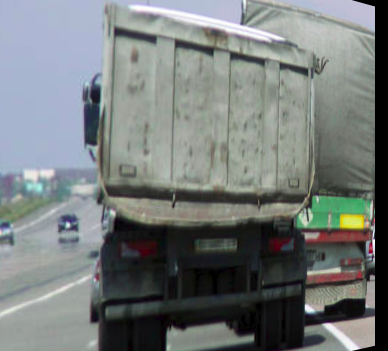
\includegraphics[width=0.7\linewidth]{imgs/truck_example/truck_rr}
\end{subfigure}
\begin{subfigure}{.19\linewidth}
  \centering
  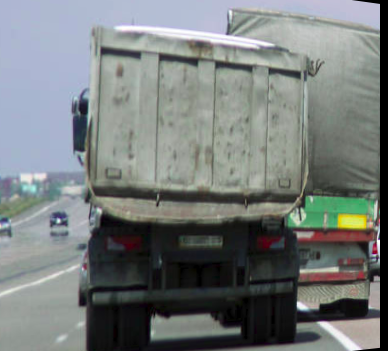
\includegraphics[width=0.7\linewidth]{imgs/truck_example/truck_r}
\end{subfigure}
\begin{subfigure}{.19\linewidth}
  \centering
  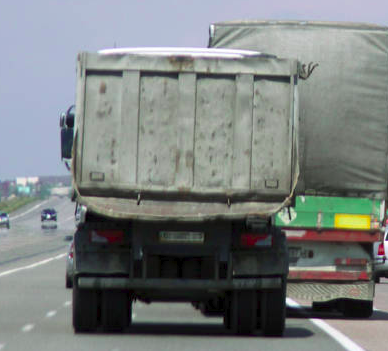
\includegraphics[width=0.7\linewidth]{imgs/truck_example/truck_c}
\end{subfigure}
\begin{subfigure}{.19\linewidth}
  \centering
  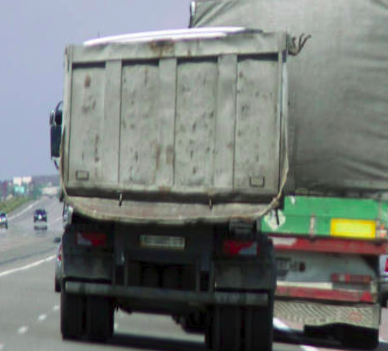
\includegraphics[width=0.7\linewidth]{imgs/truck_example/truck_l}
\end{subfigure}
\begin{subfigure}{.19\linewidth}
  \centering
  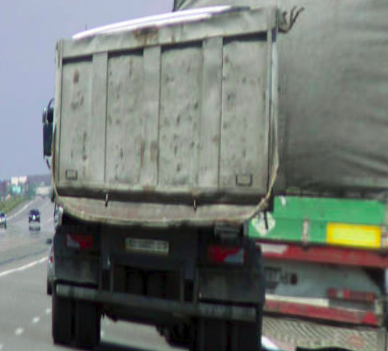
\includegraphics[width=0.7\linewidth]{imgs/truck_example/truck_ll}
\end{subfigure}
\caption{A truck from multiple synthetic perspectives}
\label{fig:truck_perspectives}
\end{figure}

While these image transformations are not sufficient enough to protect against other environmental influences, they nevertheless increase the robustness of the adversarial attacks and simulate a real-world usage.

\subsection{Robust Physical Perturbations}\label{subsec:robustphysical}

The Robust Physical Perturbation (RP$_2$) was introduced by \citet{eykholt2018robust} and defines the following minimization problem:
\footnote{The corresponding GitHub repository can be found in \cite{rp2repo}}

\begin{equation}
\argmin_\delta ||M \cdot \delta||_2 + J(F(x + M \cdot \delta), t)
\end{equation}

where $x$ is the input image and $\delta$ is the perturbation. Instead of using the logits, the output $F$ of the classifier is utilized and then passed to the loss function $J$ along with the target $t$. Although this is not quite as sophisticated as the Carlini and Wagner attack in Equation \ref{eq:cw_general}, conceptually both formulations are quite similar.

What differentiates this attack -- and what made us include it in our solution -- is the notion of a mask image $M$. 
This is a black-white image used to limit the perturbation to a specific area of the source image: White areas are modifiable in the source image, black areas are left unchanged.

The original method contains a few additional operations such as a Non-Printability Score (NPS) and calculating the mean over multiple transformations -- like we adapted for our modified Carlini \& Wagner attack.
However, we did not receive favorable results with these additional terms and subsequently removed them from the optimization.
Thus, we focused on the most important aspect of this attack, which is the ability to define a masking on the image.
This enables an attacker to define a graffiti-like perturbation.

In the original paper, this was used to reliably cause a neural network into misclassifying physical stop signs.
The InformatiCup explicitly excluded the misclassification of traffic sign images from the competition.
Yet we think this is a dangerous threat to autonomous driving, and worth mentioning, as attacks can be hidden in graffiti-like perturbations as shown in Figure \ref{fig:stopsign}.

\begin{figure}
\centering
\begin{subfigure}{.19\linewidth}
  \centering
  
\includegraphics[width=0.7\linewidth]{imgs/stopp_to_7}
\end{subfigure}
\begin{subfigure}{.19\linewidth}
  \centering
  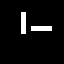
\includegraphics[width=0.7\linewidth]{imgs/stop_abstract}
\end{subfigure}
\begin{subfigure}{.19\linewidth}
  \centering
  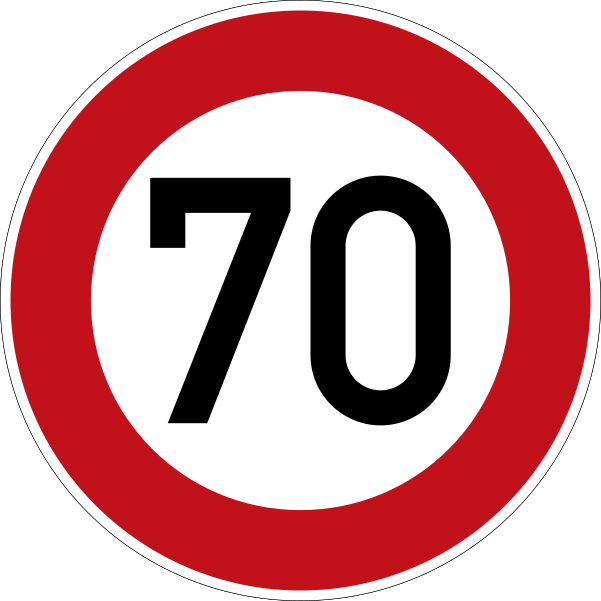
\includegraphics[width=0.7\linewidth]{imgs/7_real}
\end{subfigure}
\caption{Stop-sign (left) which is misclassified as 'Zulässige Höchstgeschwindigkeit (70)': 99.10\%, mask image (center) and true class image (right) for comparison}
\label{fig:stopsign}
\end{figure}

\subsection{Software Development}\label{subsec:sw_development}
The development velocity, code quality and maintainability of a program are heavily dependent on applying software development techniques properly.
But also, these techniques serve the developer and not vice versa which is why we chose an appropriate degree of sticking to given techniques versus being unrestrictedly productive.
Though, given the overall situation of having too little time for too many possible features, we had to plan a suitable architecture and preselect a set of features we would like to implement on the system level.
We identified trying to implement too many features as the greatest risk for our project, which may result in a lack of focus and an overall mediocre software quality.
Since on the other hand planning everything in advance is hardly possible, we decided to employ a flexible software design and pursue a more agile approach for the integration and component level.
Employing a clear separation between the main components, we were able to focus on each system component separately and to achieve the primary goal of a successful misclassification first and to then re-evaluate which exact feature set is still realizable in the remaining time.
The final set of functional system requirements is as follows, being sorted from most to least important:
\begin{enumerate}
	\item[1.] \textbf{Misclassification}
	The software shall be able to reproducibly generate adversarial examples that are classified as traffic signs by the remote model.
	\item[2.] \textbf{CleverHans Integration}
	The software shall incorporate an interface to the CleverHans library and shall use it for attacking a model. Custom attack modifications shall be implemented using the same interface.
	\item[3.] \textbf{Website}
	The software shall provide a user-friendly front end in the form of a website.
	\item[4.] \textbf{Docker}
	The software shall be distributed using docker.
\end{enumerate}

This methodology ensured a fully functional business logic before spending time on optional tasks.
Due to the small team size of two people, we refrained from creating time-consuming documents like a formal specification and decided to meet up at least once a week to reason about the current state and which steps to take next.

When working with multiple developers on the same code base, there must be a defined flow for how to implement new features and integrate them into the code base.
We decided to use git as a source code management system and to follow the \enquote{git flow}~\footnote{This concept has been initially presented in a blog post \cite{gitflow} but has found broad application under practitioners since then.}.
A basic concept of this flow is to employ a master branch for releases, an integration branch for merging new features and short-living topic branches for the actual feature implementation.
We refined this by a custom merging strategy which is further detailed in the next subsection.

\subsection{Software Testing}\label{subsec:sw_testing}
Software testing defines a set of techniques to ensure code quality and the coherence of specification and implementation.
Applying meaningful tests reduces the technical debt in the software's life cycle and therefore decreases the time spent on fixing errors as well as the amount of unknown software bugs.
Which exact techniques to apply must be decided for each project individually and depends on multiple factors like whether there are stakeholders interested in the outcome of a test and the benefit cost ratio.
For example, setting up an extensive framework for regression testing is not sensible in our context because there is only a single release version, after which there won't be any further releases requiring a regression.
Even unit tests do not fit our project very well because of the constantly changing code base which would incur the cost of permanently adjusting the test cases and re-evaluating if they are still meaningful.
Also, having no clearly defined requirements, it is not possible to derive a test plan and specification, rendering most testing approaches ineffective.
We therefore restricted ourselves to the following three testing techniques which we found appropriate in our context:
\begin{description}
	\item[Informal Code Review] This is a form of static testing which we applied before merging new features. To maintain a high development velocity, we chose the following flow: For a finished feature, the code author notifies the reviewer who then checks out the feature branch, reviews the changes and executes the code. The reviewer accepts or rejects the changes depending on potential open issues. On acceptance, the branch is merged and sent back for re-iteration on rejection. The reviewer also has the opportunity to ask for a peer review if there are many open questions or if the amount of changes is too large.
	\item[Peer Review] For bigger sets of changes, we held dedicated sessions in which the reviewer examined each change, pointing out discrepancies and asking questions. The code author then provided an explanation or noted this aspect as an open issue. After solving all issues and implementing the fixes, the reviewer checked it again before merging in an informal review.
	\item[Scenario-based Testing] This testing technique applies to the system level and defines scenarios to be tested. We identified this as vital to ensure that all components are well-integrated and that there are no unforeseen errors at the end. Testing scenarios helps ensuring a good user experience which is our main non-functional requirement in the context of this competition. The test report can be found in Appendix~\ref{app:scenariotest}.
\end{description}
Enforcing this testing strategy, we were able to develop with a high developing velocity\footnote{We performed a total of ca. 230 commits and an average of $1.35$ commits per day and team member (metrics taken from our git repository over the whole span of the project).} while maintaining a reasonable code quality.
